\documentclass[10pt,twocolumn,letterpaper]{article}

\usepackage{cvpr}
\usepackage{times}
\usepackage{epsfig}
\usepackage{graphicx}
\usepackage{amsmath}
\usepackage{amssymb}

% Include other packages here, before hyperref.

% If you comment hyperref and then uncomment it, you should delete
% egpaper.aux before re-running latex.  (Or just hit 'q' on the first latex
% run, let it finish, and you should be clear).
\usepackage[pagebackref=true,breaklinks=true,letterpaper=true,colorlinks,bookmarks=false]{hyperref}

% \cvprfinalcopy % *** Uncomment this line for the final submission

\def\cvprPaperID{****} % *** Enter the CVPR Paper ID here
\def\httilde{\mbox{\tt\raisebox{-.5ex}{\symbol{126}}}}

% Pages are numbered in submission mode, and unnumbered in camera-ready
\ifcvprfinal\pagestyle{empty}\fi
\begin{document}

%%%%%%%%% TITLE
\title{UFo - Coupling Uncertain Active Constellation Models with \\
Cascaded Forest Predictors for Sematic Segmentation}

\author{First Author\\
Institution1\\
Institution1 address\\
{\tt\small firstauthor@i1.org}
% For a paper whose authors are all at the same institution,
% omit the following lines up until the closing ``}''.
% Additional authors and addresses can be added with ``\and'',
% just like the second author.
% To save space, use either the email address or home page, not both
\and
Second Author\\
Institution2\\
First line of institution2 address\\
{\tt\small secondauthor@i2.org}
}

\maketitle
%\thispagestyle{empty}

%%%%%%%%% ABSTRACT
\begin{abstract}
We consider the task of model-based semantic segmentation. The model is described by a constellation model of parts that are represented by active shape- and appearance models. We term this an active constellation model. As a running example we utilize a 21-part, chain-based spine model of a zebra fish observed in microscopic images. The prevailing approach to solve this task is to first generate pixel-independent features for each part, e.g.\ via a cascaded decision forest predictor, which are then fed into an MRF-based model-fitting objective to infer the optimal MAP solution of the constellation model. Our key contribution is to abandon this static, two-stage approach and mix feature generation and model-based inference in a new, more flexible, way. In particular we interleave the cascaded forest predictors with inference steps for the model-fitting. A key finding is that “uncertain” model-outputs at intermediate stages of the cascade, in the form of part-based marginals, are essential for best performance. This is because, on one hand the semantic segmentation is guided by the model, and on the other hand correct solutions, which are different to intermediate MAP solution, can still be found. We validate our findings with an in-depth study of alternative inference steps, including popular geodesic smoothing as well as MAP inference. %, and alternative output generation steps, including max-marginals. 
We believe that our findings are not only relevant for other types of constellation models but, more generally, for the recent trend of combing deep learning models with physically-motivated structured models. 
\end{abstract}

\begin{figure}
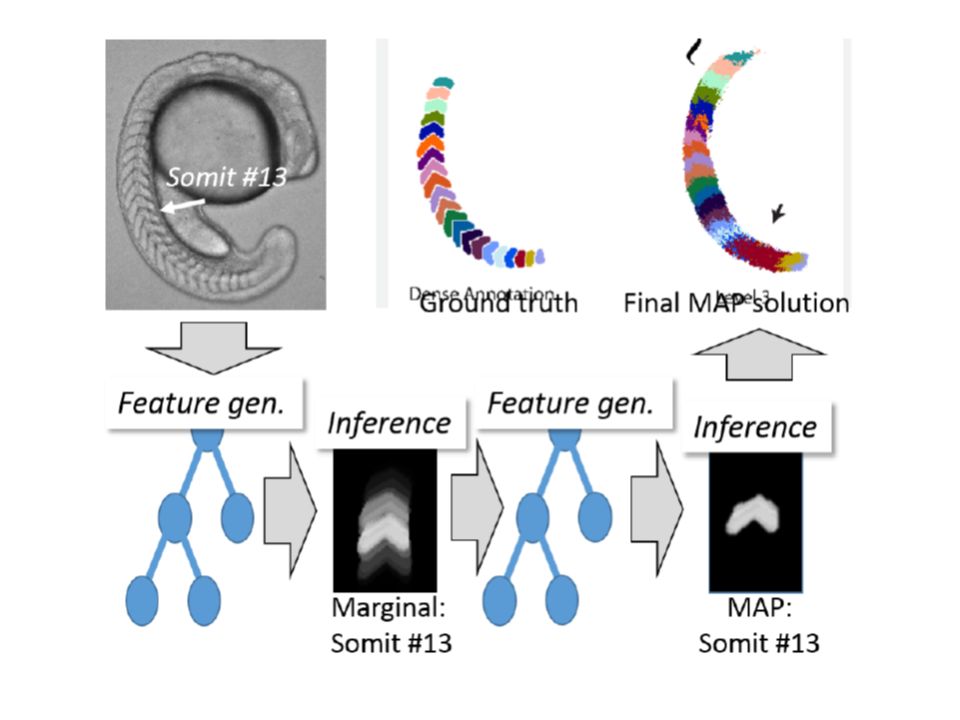
\includegraphics[width=0.5\textwidth]{Teaser.png}
\caption{Teaser figure.}
\label{fig:teaser.}
\end{figure}


\section{Introduction}
Many tasks in computer vision have as input an image and as output a dense labeling, where each pixel is assigned one out of many pre-defined classes. An example is a sematic segmentation of a person in an image, where each pixel is assigned a label such as “background”, “left leg”, or “head”. 
To solve this task, two major trends in computer vision have played an important role in the last decades.  The first, well studied, trend is to infer the MAP or Max-Marginal solution in a so-called structured model, such as a Conditional Random Field (CRFs). Here structure models mean that neighboring pixels in an image do not make independent decisions, e.g. neighboring pixels are likely to take the same label. The form of the potential functions in the structure model is based on two sources of information.  On one hand it is guided by {\bf physical principles}, such as the kinematics of a person. On the other hand, in many applications the potential functions have to be derived from the input data itself. This brings us to the second, more recent, major trend in computer vision, namely learning deep models, such as CNNs~\cite{NIPS2012_4824}, Auto-Context Models~\cite{AutoContext2008,PoseMachinesECCV2014} or Cascaded Forest predictors [DTF,RTF,GeoF,Uwe]. These models play the role of learning a complex non-linear mapping from images to features which are relevant for the task at hand. 

The classical example of how to use these trends from semantic segmentation (see e.g.\ []) is to train a deep model, e.g. cascaded forest predictor, from image data that gives for each individual pixel a distribution over class labels. These class-label distributions define the unary potentials in the CRF, where the pairwise potentials, e.g.\ on a 4-connected grid, are gradient-weighted Potts-model terms. This modelling framework is however very static: first features are generated and then the dense labeling, e.g. MAP solution, is inferred. For instance, in order to optimize test-time performance, the first question is about the appropriate run-time trade-off between generating features and performing inference. Oftentimes, MAP inference is NP-hard and considerable more time is spend on MAP inference than feature generation. On the other hand, better features lead often to models with potential simpler MAP inference problems, since they relate to stronger unary potentials. This simple discussion motivates that one has to think of the two steps in a more holistic fashion – which is the goal of this work.

In this work we are concerned with new ways to interleave feature generation, via deep learning models, and inference in structured models, guided by physical principles. This is in our view one of the most crucial questions for making a step forward in dense labeling tasks. For this we will consider the task of semantic segmentation with an active constellation model; That means that the parts are defined via active shape and appearance models~\cite{CootesAAM2001}. Motivated by recent work~\cite{UweCVPR2013} on cascaded regression Forests with interleaved Gaussian Conditional Random Fields we suggest a cascaded pipeline that is illustrated in Figure 1. The most important aspect of this cascade is the question of what to infer from the constellation at intermediate stages of the cascade. Various ideas come to mind: Marginals or MAP solution of the MRF-based constellation model. These are opposed to model-agnostic geodesic smoothing as suggested by~\cite{GeoForests2013}. One of the main aspects of this work is to study these trade-offs. We see that for model-based segmentation of spines in zebra-fish, soft marginals are a clear winner. The reason is that individual parts (so-called somites) are highly ambiguous with respect to shape and appearance, hence only the relative spatial arrangement can disambiguate this situation. Marginals help to not commit to a wrong solution in the early stages of the cascade.
To summarize, we claim the following three {\bf contributions}:
\begin{itemize}
\item In the field of model-based semantic segmentation we are the first to interleave feature generation and model-based inference. We show that this boost performance considerably, compared to not cascading. Note, related hierachical appraoches~\cite{CootesECCV2012RRFandSSM,CootesFemurTMI2013} focus on speed not quality that comes form feature generation. 
\item We show, for the first time, that probabilistic inference gives a major (6\%) boost in performance in cascaded MRF-Forest-based models. This is compared to standard MAP inference (as e.g.\ in \cite{Glocker2013,SeifertAnatomicalSPIE2009,TeethMICCAI2012}) and model-agnostic geodesic smoothing~\cite{GeoForests2013}. 
\item We are the first to tackle spine detection in zebra fish, where we achieve an overall average Dice score of 82\%.
\end{itemize}



%%%%%%%%% BODY TEXT
\section{IntroductionOld}
The idea is to do "model-based smoothing" of the output of a Random Forest classifier, in an iterative or cascaded fashion.  This generalizes the idea proposed by GeoF~\cite{GeoForests2013}, which does "image aware" smoothing, using Geodesic distances. 
%
Another way to look at this is that we want to mix discriminative (discr) and generative models (gen), in a smart way.  E.g., The discr model initializes the gen model in the right search space, the gen model then refines this initialization.  This process is iterated while simultaneously increasing the "confidence" in the discr model output. 

Our contributions: 
%
(1) Use Active Appearance Model and HMM for "`image aware"' smoothing in a RF cascade. 
Closest works: 
First, AutoContext~\cite{AutoContext2008}, but they don't do any smoothing. 
Second, GeoF~\cite{GeoForests2013}, but they don't use a generative model for smoothing. 
Third, Glocker, either with Classification Forests~\cite{Glocker2013} or Regression Forests~\cite{Glocker21012}, but they do not run a cascade. 
%
%(2) Tree weighting based on smoothing. Can be combined with any kind of smoothing. Idea: rate the trees of a forest: who agrees most with the smoothed output? This way, ...
%%

Additional Literature.
\begin{enumerate}
\item Deformable Templates Guided Discriminative Models for Robust 3D Brain MRI Segmentation.~\cite{BrainSeg2013}  Liu et al.  2013: Uses generative model to "refine" features in a cascaded discriminative classifier.
\item Uwe's hint \cite{Denzler2012}: As Time Goes by -- Anytime Semantic Segmentation with Iterative Context Forests
\end{enumerate}


\section{Background / Related work}

To be structured. The current entangling of Background and additional references does not work. 
Goal: put rel. work in Introduction; Give as much as we like background on RF to fill space (low priority!!! -- as a minimal solution just refer to Breiman), and do a more thorough background on AAMs (0.5page)

\paragraph{RF. }
We assume that the reader is familiar with the general concept of Random Forests [Breiman]. Filter Bank, Classification Forest, offset and difference features. 

\paragraph{Cascading. }

Cascading with Model Fit: DTF, RTF, GeoF

\paragraph{Constellation Models/Inference. }
CRF, probabilistic inference.

\emph{Related work on Constellation models and Forests: }

Spine: Glocker~\cite{Glocker2013}

Body parts: Auto Context~\cite{AutoContext2008}, "`Pose Machines"' ECCV 2014~\cite{PoseMachinesECCV2014}

Abdominal images: GeoF~\cite{GeoForests2013}, and GeoF at IPMI 2011~\cite{CriminisiAbdominalIPMI2011}: "'Entangled Decision Forests and their Application for Semantic Segmentation of CT Images"'. Seifert SPIE: Marginal space learning classifier plus MRF~\cite{SeifertAnatomicalSPIE2009} 

\emph{Related work on Constellation models of self-similar structures: }

Spine: (Glocker) Klinder (SSM)~\cite{Klinder2009471}: Generalized Hough Transform as detector

Dental: our MICCAI 2012~\cite{TeethMICCAI2012} (Generalized Hough Transform + SSM as detector)

Worm~\cite{WormMiccai2014}


\paragraph{AAM. Dave, please work on this. Should be 0.5p max. Terminology as in Cootes papers.}
Active appearance models (AAMs)~\cite{CootesAAM2001} are linear, generative, parametric models of shape and appearance that are learned (PCA) from training data.  Fitting an AAM is a non-linear optimisation problem, that is done via incremental updates to fitting parameters.  Importantly, AAMs can be easily extended to include priors on the model parameters (see also~\cite{BakerAAM2004}).  

Shape Model:

\[s = s_0 + \sum_{i=1}^n p_i s_i\]

where s is a vector of x,y coordinates of the landmarks that define the shape.  From PCA, $s_0$ is the mean shape, and $s_i$ are n eigenvectors corresponding to the n largest eigenvalues.  Not shown here is that the training data is first noramlised using a Procrustes analysis using a global shape normalising transformation (in our case, a similarity transform) to avoid modeling this variation in the linear model.

Appearance Model:

\[A(x) = A_0(x) + \sum_{i=1}^m \lambda_i A_i(x)\]

Analogous to shape model. $A_0$ and $A_i$ are computed from PCA on a set of \emph{shape normalised} training images, which have been warped onto the base-mesh $s_0$.  Shape normalizing is a key benefit of AAMs (compared to e.g. Eigen-faces), and leads to more compressed PCA representation.

To create a model instance, create an image A(x) (defined by $\lambda$) on the base-mesh, and then warp it to s (defined by p).  Warping is done using a thin-plate spline, parameterized by the set of landmarks, $s_0$ and s.  This defines the unique warp parameterised by p, called W(x;p).

Fitting criteria:

\[Error = A_0(x) + \sum_{i=1}^m \lambda_i A_i(x) - I(N(W(x;p);q)) \]

where N(x;q) is the similarity transform, parameterized by q, and the cost is typically the sum of squared errors over the shape normalized patch.

\[Cost = \sum_{x \epsilon s_0} [Error]^2 \]

Final note, the most efficient fitting routine [] actually "projects out" the appearance variation (from the Error image), and simply solves for the parameters of the transformation: p,q.  If you keep one shape parameter (n=1), this leads to a 5 parameter model.


One can add priors on the model parameters, as follows:

\[ \sum_{x \epsilon s_0} [A(x) - I(N(W(x;p);q)]^2 + \sum_{i=1}^K F_i^2(p,q) \]

If $F_i(p,q)$ is quadratic, this can be interpreted in the Bayesian framework as Gaussian Regularization.  There's also a clear way to "ramp" the importance of the priors as:

\[ F_i^2(p,q) = r[(p-p_0)^2+(q-q_0)^2]) \]

where r is the parameter that captures how much we trust the discr model output (this could be learned). 

Note, adding priors doesn't slow down the code too much.  You can still use the same fitting algorithm, there's just some extra computation in each loop.

\emph{Related work on SSMs and Random Forests: }

Cootes Femur TMI 2013~\cite{CootesFemurTMI2013}

Cootes Regression Forest + SSM ECCV 2012~\cite{CootesECCV2012RRFandSSM}



\section{Method. Dave, please work on this.}
\emph{Cascaded RF Interleaved with Probabilistic Generative Constellation Model Inference.}

Problem: Given an image, get a pixel-wise multi-classification. 

We propose the following pipeline for model-based semantic segmentation, as layed out in Figure~\ref{fig:pipeline}: 
%
First, we generate probability maps for each class with a random forest classifier.
%
Second, we generate many part ("`segment"') proposals for each class, with the help of Active Appearance models. 
(Each proposal is a binary segmentation.) (cf.\ Sec.\ \ref{subsec:hyps}). 
%
Third, we perform probabilistic inference in a constellation model to weigh part proposals (cf.\ Sec.\ \ref{subsec:weightsAndFusion}). 
%
Fourth, we feed the resulting "`smoothed"' probability maps, together with the original image, features, and RF output, into a next level of random forest classifier. 
%
To generate a resulting labeling, one can take the class with max probability according to the RF output of the last level, or the "`smoothed"' output of the last level. 


\begin{figure*}[t]
\begin{center}
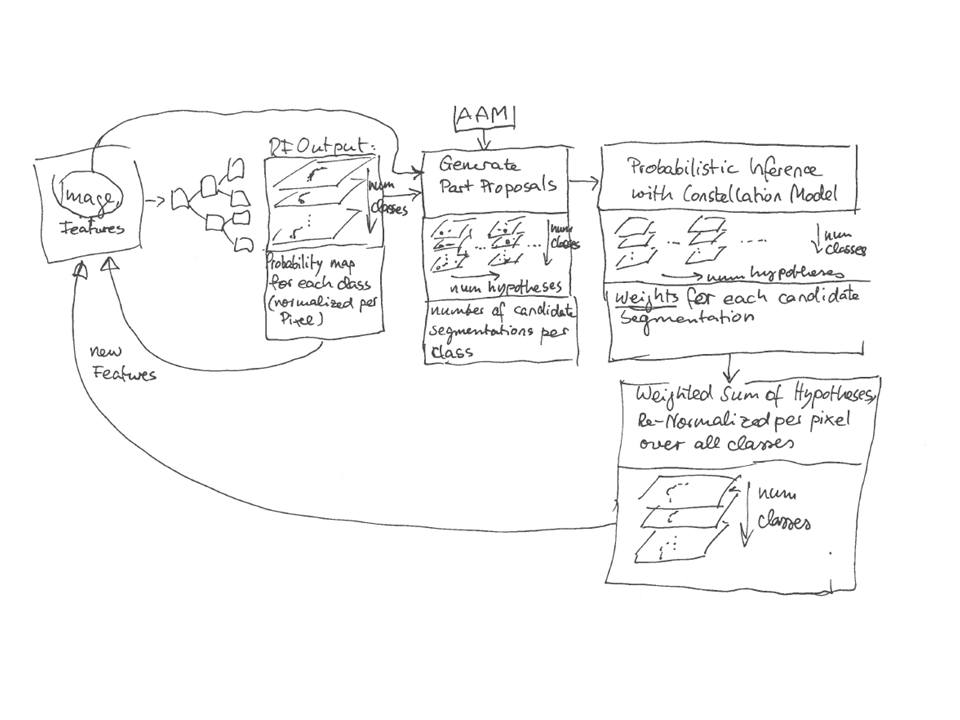
\includegraphics[width=\textwidth]{Pipeline.png} %&[trim=0cm 2cm 0cm 1cm,height=0.2\textheight]
\caption{Pipeline.}
\label{fig:pipeline}
\end{center}
\end{figure*}

\subsection{Generating Part Proposals}
\label{subsec:hyps}

(1) Compute Centroid of RF output, per class, via mean shift. 

(2) Fit average constellation model (i.e.\ static set of landmarks) to these centroids (sum of squared distances; global similarity transform). In our application, this is enough to define an approximate orientation of the part. 

(3) Sample around centroids to get a set of location initializations. 

(4) Run AAM (with a part-specific model) from all inits. Each run results in a binary segmentation, together with a cost for the fit (cf.\ Eq.\ \eqref{}. 

\subsection{Weighting and Fusing Part Proposals}
\label{subsec:weightsAndFusion}

Pairwise MRF.

Nodes: $c\in \{1..n_C\}=:C$=Classes

Labels: $l\in \{1..n_L\}=:L$=Part Proposals. (Here: Same number $n_L$ for all classes.)

Unaries: $\phi_c(l)$=AAMFit and integrated RF output

Binaries: $\psi_{c,b}(l,k)$ =Learnt from Training Data

By the above method, a number of model instances are initialized and fit, for each class.  Each model instance has a cost associated with its fit.  Use these costs as unaries in a Markov Chain Model.  The pair-wise energy comes from statistics on the relative position of neighboring segments in the training data.  This is exactly what Glocker did already; however, we do probabilistic inference (rather than MAP inference) and keep all the marginals.

Recall, since we initialized many AAMS for fitting, and did probabilistic inference over all of these solutions, we have multiple masks each with its own probability.  For each class c, compute a weighted average:

\[ P_c(x,y) = \frac{1}{Z(x,y)} \cdot \sum_{l\in L} p_c(l)\cdot H_{l,c}(x,y) \]

where there are L model instances initialized (for ease of notation, same number for all classes), $H_{l,c}$ is the binary mask that represents the $l$-th proposal for class $c$, and $p_c(l)$ is the marginal probability of model instance l being the true segmentation of class c, as obtained by probabilistic inference, and $Z(x,y)$ serves for pixel-wise re-normalization. I.e., $Z(x,y)=\sum_{c\in C}\sum_{l\in L} p_c(l)\times H_{l,c}(x,y)$.

We call $P_c$ the \emph{smoothed probability map} for class $c$. 

\subsection{Parameters}
... to be put into respective equations spread everywhere...
\begin{itemize}
\item n: \# of shape modes
\item m: \# of appearance modes
\item r: trust in discr output
\item S: \# of model instances that are initialized for fitting
\item g: \# of grad descent steps
\end{itemize}

\section{Results}
Approach: Cascade interleaved with "`smoothing"'. 
Evaluation: Different kinds of "`smoothing"', each with different kinds of outputs.

Dataset: 32 images of developing zebra-fish. Task: Semantic segmentation of 21 somites (i.e.\ developing vertebrae).

\paragraph{Ours. }
AAM with probabilistic inference 

\paragraph{Auto Context. }

\paragraph{GeoF. }
The simplest way to generate a smoothed RF Output is to re-use the Geodesic smoothing idea from Criminisi.  Let:

\[ Q(x; M, \nabla I) = \min_{x'} (\delta (x,x') + \nu M) \]

and $\nu$ is some free parameter.  Note, x and x' are two points in the image. $M(x') = 1 - p(c|v(x'))$, where v(x') is the feature vector at pixel x'.  Then the smoothed RF output is calculated as:

\[ g(c|v(x)) = \frac{1}{Z} p(c|v(x)) e^{\frac{-Q(x;p(c|v(\Omega)),\nabla J)^2}{\sigma ^2}} \]

This accomplishes smoothing in quite an indirect way, as a competition between different possible class labels for a given pixel, mediated by the normalization Z.  \textbf{It would be interesting to think of more direct ways to implement smoothing.}  However, within this framework, we could just replace the geodesic distance function and the definition of M.


\paragraph{MAP Inference. }

\begin{figure}[t]
\begin{center}
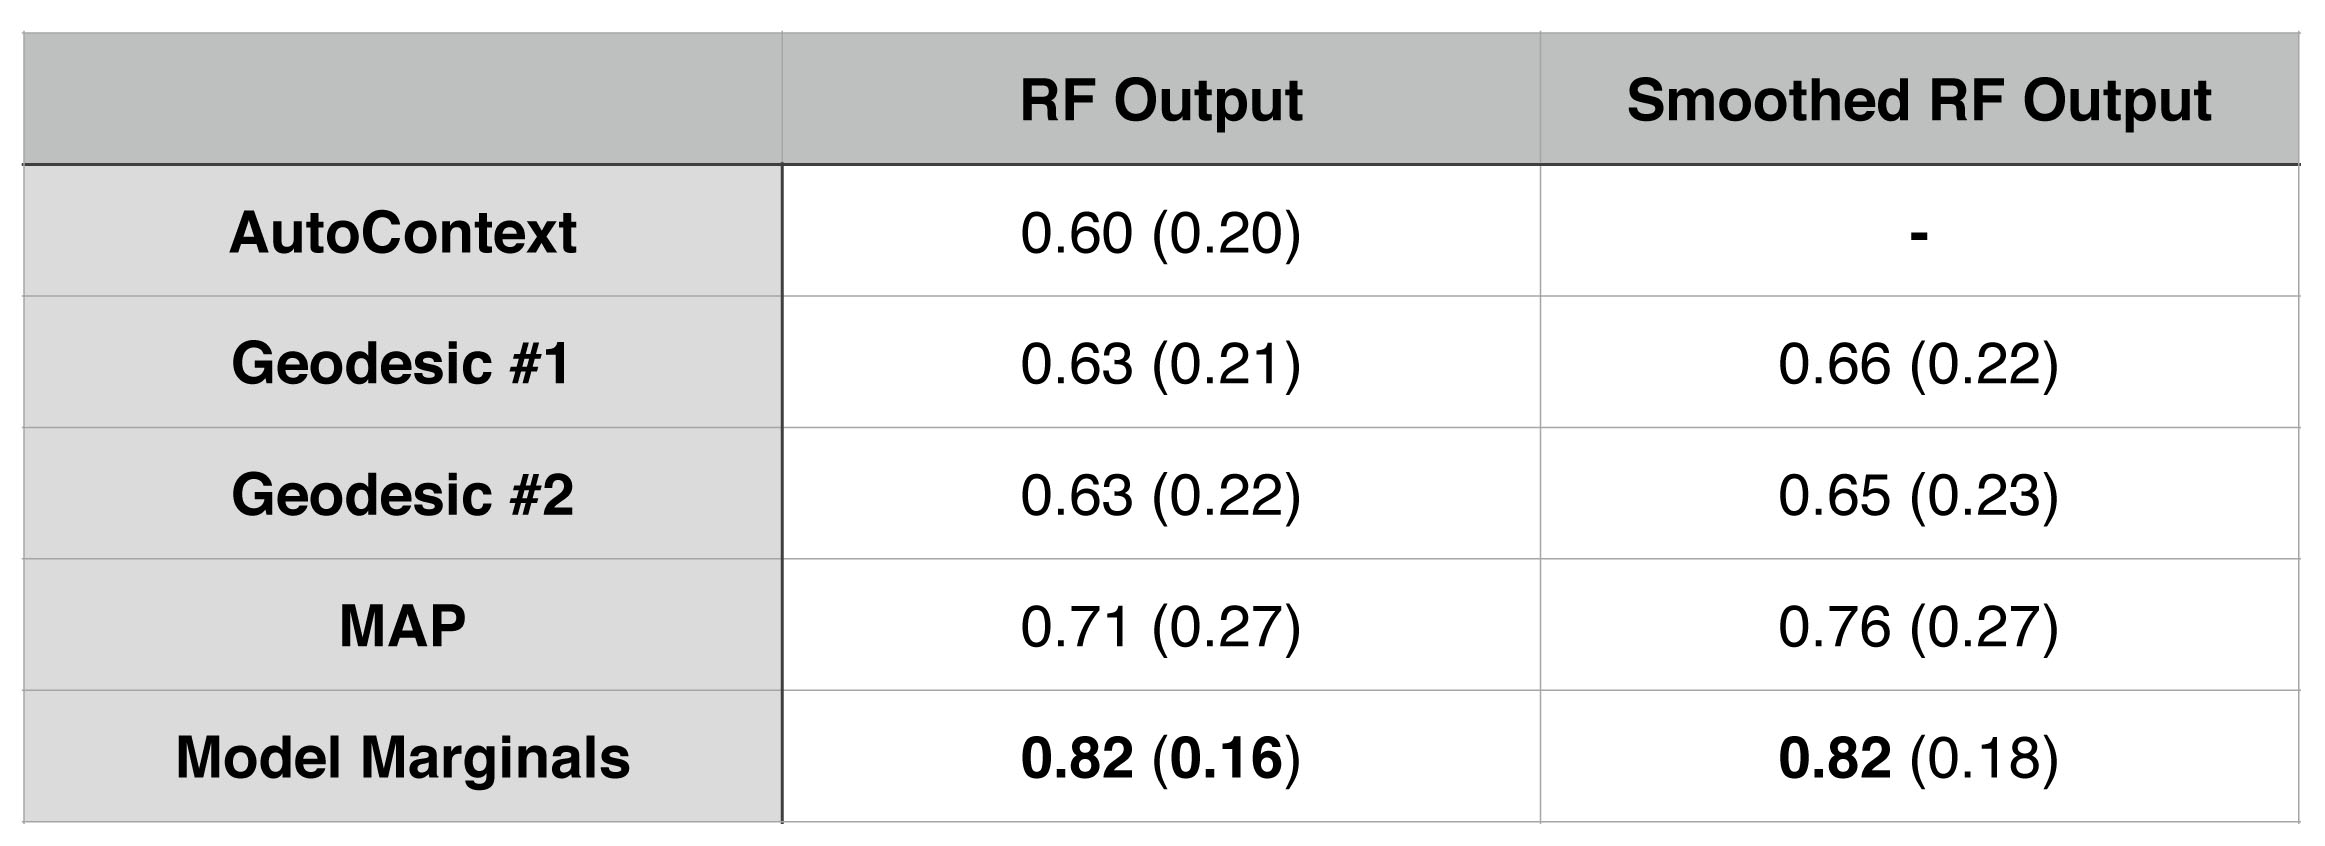
\includegraphics[width=\columnwidth]{TableDiceScores.jpg} %&[trim=0cm 2cm 0cm 1cm,height=0.2\textheight]
\caption{Evaluation on 32 datasets. Dice Scores on all 21 Somites: Mean and standard deviation (in brackets).}
\label{tab:results}
\end{center}
\end{figure}

\begin{figure}[tb]
\centering
\small
\begin{center}
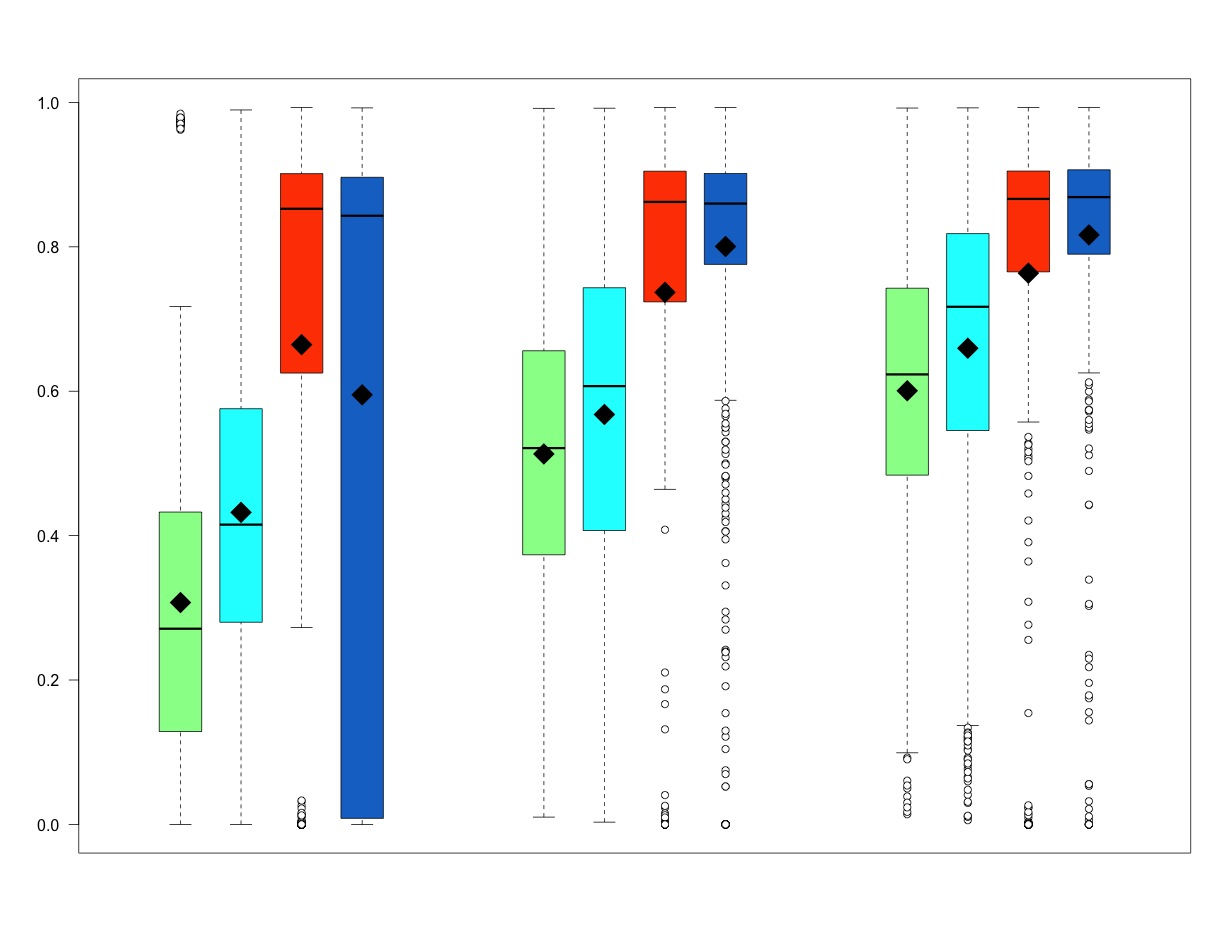
\includegraphics[width=\columnwidth]{Cascade.jpeg} %&[trim=0cm 2cm 0cm 1cm,height=0.2\textheight]
\end{center}
\label{fig:boxplots}
% \vspace{-2mm}
\caption{3 level cascade. Segmentation accuracy of 4 methods after each level: RF output (green), GeoF (cyan), MAP (red), Ours (blue). For every method at every level, Dice scores of 21 somites in 32 images, i.e.\ 672 scores, are visualized as a \emph{box plot}~\cite{chambers1983graphical}. A colored box spans from lower to upper quartile, i.e.\ the inter-quartile range. I.e.\ 50\% of the data points lie within the box. The horizontal bar within the box depicts the median. The black diamond depicts the mean. Whiskers depict the outlier-free data range. Circles depict outliers. Outliers are defined as data points beyond median $\pm$ 2 inter-quartile ranges. }
\end{figure}

\section{Discussion}
Ours is the best :)

\paragraph{Cascading Helps!}
... performance goes up over levels. Boxplots!

... "`traditional"' MAP after one level sucks. 

\paragraph{Smoothing Helps! Model-based Smoothing Helps Best!}
... Auto Context $<$ GeoF $<$ Model Based. Reason: More Specific Prior knowledge...

\paragraph{Uncertainty Helps!}
... Probabilistic inference considerably outperforms MAP inference (6\% better). Reason: With Prob.\ inference, cases can be rescued if not caught after first level (i.e.\ "`at first site"'). Show some rescue cases. 

We also tried MAP after third level. Once all cases are rescued, MAP is fine (performs equally -- state numbers). BUT NOT EARLIER!



{\small
\bibliographystyle{ieee}
\bibliography{somites2014}
}

\end{document}
